
\subsection{Experimental Setup}
\label{subsec:setup}

We use the publicly released final Pythia-410M-deduped checkpoint \citep{biderman2023pythia} as our base model and fine-tune on a randomly sampled 50K-subset of OpenWebText (filtered to sequences with $\geq$256 non-padding tokens).
Starting from the pretrained checkpoint (generation~0), each subsequent generation fine-tunes on synthetic text produced by the previous generation, for a total of 10 recursive generations.
At each generation we compute the spectral indicators from \S\ref{subsec:spectral_metrics} on 1K held-out last-layer embeddings, paired with three downstream metrics: perplexity, HellaSwag accuracy (0-shot), and distinct-4.
These three metrics (language modeling capability, natural language understanding, and generation diversity) cover the primary evaluation dimensions accessible to a 410M-parameter model.
Training hyperparameters and compute details are in Appendix~\ref{app:training_details}.

For the mixing comparison (\S\ref{subsec:phase1}), we evaluate three strategies:
(1)~\textbf{pure collapse} ($r_t{=}0$),
(2)~\textbf{fixed mix} ($r_t{=}0.50$), and
(3)~\textbf{adaptive} ($k{=}10$, Eq.~\ref{eq:controller}).
To construct the collapse trajectory map (\S\ref{subsec:phase_diagram_exp}), we additionally evaluate fixed mixing at $r \in \{0.2, 0.25, 0.3\}$.

\subsection{Spectral Collapse Characterization}
\label{subsec:phase0}

Table~\ref{tab:phase0} reports spectral and downstream metrics across 10 recursive generations, which reveal a three-phase structure.

\paragraph{Phase I: Spectral Decompression (Gen~0--2).}
$r_{\text{eff}}$ rises from 417.55 to 496.2 (+18.8\%) and SLV from 2366.7 to 2468.0 (+4.3\%), while $\sigma_1$ drops from 1942.8 to 718.7.
The peak at Gen~2 is consistent across all three seeds (Figure~\ref{fig:seed_variability}; SLV coefficient of variation (CV) $< 1.3\%$ at all generations; full per-generation statistics in Appendix Table~\ref{tab:pergen_variance}).\footnote{With only $n{=}3$ seeds, bootstrap CIs ($B{=}10{,}000$, percentile method) provide descriptive summaries of observed variability; actual coverage may fall below nominal.}
However, this decompression does not indicate improved model quality: HellaSwag drops 8.0\% and distinct-4 falls 31.6\% during the same interval (Figure~\ref{fig:slv_ppl_decoupling}), and SLV computation takes ${<}\,1$\,s vs.\ ${\sim}$70\,min for benchmarks.

\begin{figure}[t]
\centering
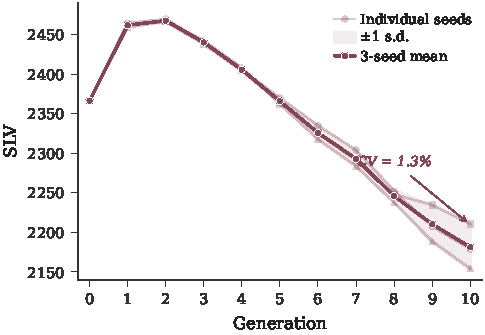
\includegraphics[width=\columnwidth]{figures/seed_variability.pdf}
\caption{Cross-seed reproducibility of SLV under pure-synthetic training ($r{=}0$). Thin lines: individual seeds (42, 43, 44); thick line: 3-seed mean; shaded band: $\pm$1 s.d. The coefficient of variation remains below 1.3\% at all generations; spectral collapse follows a deterministic trajectory.}
\label{fig:seed_variability}
\end{figure}

\begin{figure}[t]
\centering
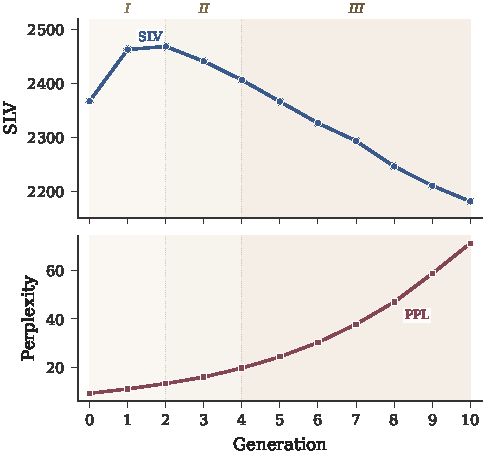
\includegraphics[width=\columnwidth]{figures/slv_ppl_decoupling.pdf}
\caption{SLV (top) and perplexity (bottom) across 10 recursive generations ($r{=}0$, 3-seed mean). In Phase~I (Gen~0--2), both metrics rise simultaneously. The SLV increase reflects distributional broadening, not model health. From Phase~III onward (Gen~4--10), the two metrics diverge: SLV declines monotonically while perplexity accelerates, which confirms that post-decompression SLV faithfully tracks structural collapse.}
\label{fig:slv_ppl_decoupling}
\end{figure}

\paragraph{Phase II: Collapse Onset (Gen~2--4).}
Both $r_{\text{eff}}$ and SLV reverse after Gen~2 ($r_{\text{eff}}$: 496.2$\to$493.6, SLV: 2468$\to$2440), marking the transition from decompression to collapse while perplexity continues its monotonic rise.
SLV's post-peak decline is sharper than $r_{\text{eff}}$'s ($-$1.1\% vs.\ $-$0.5\% in the first post-peak generation) because SLV captures distributed contraction across all spectral directions rather than the dominant ones alone.
At 1B scale, this sensitivity gap widens to a timing difference: SLV peaks one generation earlier than $r_{\text{eff}}$ (see Cross-Scale Pilot below).

\paragraph{Phase III: Accelerating Collapse (Gen~4--10).}
SLV contraction accelerates: the per-generation decline averages $-$31.0 during onset (Gen~2--4) vs.\ $-$37.4 during acceleration (Gen~4--10), with 78\% of the total peak-to-final decline occurring in Phase~III (Table~\ref{tab:pergen_variance}).
By Gen~10, $r_{\text{eff}}$ falls to 438.1 ($-$11.7\% from peak), SLV to 2181.4 ($-$11.6\% from peak), and perplexity reaches 71.0 ($+$643\%).
Concurrently, $\sigma_1$ traces a U-shaped trajectory: after dropping from 1942.8 to 718.7 during decompression, it rises to 874.6 by Gen~10 (Figure~\ref{fig:spectral_trajectory}).
This simultaneous $\sigma_1$ recovery and $r_{\text{eff}}$ decline is a geometric signature of mode collapse: representations concentrate along fewer dominant directions while the overall occupied volume shrinks.

\paragraph{Cross-Scale Pilot.}
Repeating the protocol on Pythia-1B-deduped (Gen~0--3) reproduces the decompression-onset structure: SLV rises from 2835 to 2906 at Gen~1 ($+$2.5\%) before declining to 2865 at Gen~3, while $r_{\text{eff}}$ peaks one generation later at Gen~2 (580.9 vs.\ 570.8 at Gen~1).
This one-generation SLV lead over $r_{\text{eff}}$ (absent at 410M, where both peak simultaneously) suggests that SLV sensitivity increases with model scale.
Perplexity rises monotonically throughout (8.1$\to$13.4, $+$66\%)---the same downstream-spectral asymmetry observed at 410M scale.
Full 10-generation characterization at 1B remains future work.

\subsection{Adaptive Mixing Comparison}
\label{subsec:phase1}

We evaluate the controller retrospectively by computing its signal on pre-existing fixed-ratio trajectories rather than deploying it in a closed loop; the goal is to characterize signal attenuation, not to propose operational deployment.
Under pure synthetic training, SLV peaks at Gen~2 (2468) and declines monotonically; with 50\% mixing, SLV rises to 2572 at Gen~10, with only a negligible Gen~1 dip ($\Delta_1 \approx 0.0005$, well below $\tau$).
The adaptive controller ($k{=}10$) remains silent through all ten generations.
Figure~\ref{fig:controller_signal} quantifies the signal attenuation: the maximum controller signal magnitude drops from 40.4 at $r{=}0$ to 3.8 at $r{=}0.2$ and reaches exactly zero at $r \geq 0.3$. Even moderate mixing suffices to suppress the rate-based signal~\citep{scheffer2009ews}.

\begin{figure}[t]
\centering
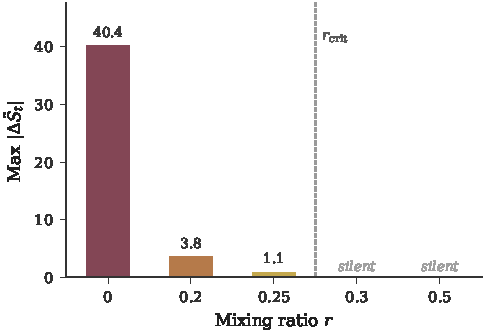
\includegraphics[width=0.85\columnwidth]{figures/controller_signal.pdf}
\caption{Maximum controller signal magnitude ($\max|\Delta\tilde{S}_t|$, $t \geq 2$) across mixing ratios. The signal drops $10\times$ from $r{=}0$ to $r{=}0.2$ and is exactly zero for $r \geq 0.3$ (``silent''), rate-based controllers are therefore ineffective.}
\label{fig:controller_signal}
\end{figure}

Despite sustained spectral expansion at $r{=}0.5$, downstream metrics degrade: perplexity increases 58\% and distinct-4 falls to .152 (below even pure collapse), reinforcing that spectral health does not guarantee model health.

\subsection{Alternative EWS Comparison}
\label{subsec:alt_ews}

We compare SLV against seven alternative collapse indicators from three signal sources: embedding geometry (RankMe, isotropy), attention weights (stable rank, spectral norm), and output distributions (token entropy, raw perplexity, perplexity growth rate).
We exclude generated-text metrics (distinct-$n$, self-BLEU) because they require full decoding (${\sim}$70\,min vs.\ ${<}\,1$\,s) and operate in output space rather than the representation space this study targets.

Table~\ref{tab:ews_main} summarizes the comparison under pure-synthetic training ($r{=}0$); full tabular data appear in Appendix Table~\ref{tab:ews_comparison}.
Only SLV and RankMe~\citep{rankme2023} exhibit a decompression peak at Gen~2 followed by monotonic decline; all other indicators change monotonically from Gen~0 and cannot distinguish collapse onset from the initial fine-tuning transient.
SLV's signal-to-noise ratio is 2.5$\times$ that of RankMe (11.8\% vs.\ 4.7\% relative change).

\begin{table}[t]
\centering
\small
\setlength{\tabcolsep}{4pt}
\begin{tabular}{@{}llcc@{}}
\toprule
Indicator & Direction ($r{=}0$) & Rel $\Delta$ & Rev. \\
\midrule
SLV         & Peak G2, mono.\ $\downarrow$ & 11.8\% & \checkmark \\
RankMe      & Peak G2, mono.\ $\downarrow$ &  4.7\% & \checkmark \\
Token ent.  & Mono.\ $\downarrow$           &  9.6\% & \checkmark \\
Stable rank & Mono.\ $\downarrow$           & 14.0\% & \checkmark \\
Spec.\ norm & Mono.\ $\uparrow$            &  8.0\% & \checkmark \\
Isotropy    & Non-mono.\ (6 rev.)           & 75\%   & \checkmark \\
Raw PPL     & Mono.\ $\uparrow$            & 704\%  & $\times$ \\
PPL growth  & ${\sim}$Mono.\ $\downarrow$   &  ---   & \checkmark \\
\bottomrule
\end{tabular}
\caption{Eight EWS indicators under pure-synthetic training ($r{=}0$, Pythia-410M). \textbf{Direction}: trajectory shape (Peak G$n$ = decompression peak at generation $n$; mono.\ = monotonic post-peak or throughout). \textbf{Rel $\Delta$}: total relative change. \textbf{Rev.}: whether the indicator reverses under $r{=}0.5$ mixing. Seven of eight reverse; raw PPL is the sole exception. Full data in Appendix Table~\ref{tab:ews_comparison}.}
\label{tab:ews_main}
\end{table}
Seven of eight indicators reverse direction under mixing (Table~\ref{tab:ews_main}, last column); raw perplexity is the sole exception.
This near-universality confirms that signal attenuation is not specific to SLV: any rate-based controller will fall silent when mixing exceeds $r_{\text{crit}}$.
SLV is the only indicator that combines decompression-phase sensitivity, post-peak monotonicity, and sub-second computation cost; it shares a metric foundation with SIGMA's $\log\det G$ ($= 2 \times \text{SLV}$; \S\ref{sec:related}).
Raw perplexity is a stronger unconditional monitor (monotonic from Gen~0, no decompression mislead) but does not reveal the spectral geometry of collapse; SLV and PPL are complementary.

\subsection{Collapse Trajectory Classification}
\label{subsec:phase_diagram_exp}

We now map SLV trajectories across mixing ratios to construct the collapse trajectory map defined in \S\ref{subsec:phase_diagram}.
Figure~\ref{fig:phase_diagram} plots SLV across 10 recursive generations for five mixing ratios; three qualitatively distinct trajectory types emerge:

\begin{figure}[t]
\centering
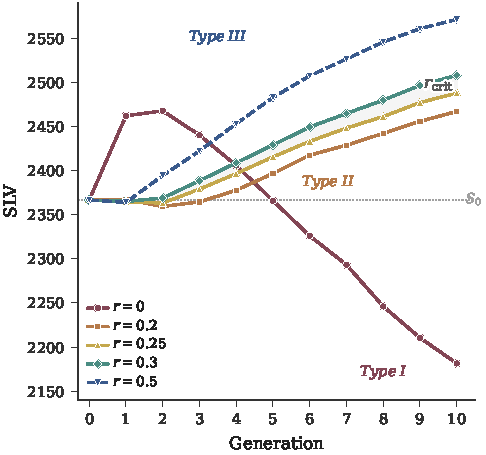
\includegraphics[width=0.92\columnwidth]{figures/phase_diagram.pdf}
\caption{SLV trajectories across mixing ratios (Pythia-410M; $r{=}0$, $r{=}0.2$, $r{=}0.25$, $r{=}0.3$: 3-seed mean, solid lines; $r{=}0.5$: 2-seed mean, dashed line). Type~I ($r{=}0$): decompression then monotonic collapse. Type~II ($r{=}0.2$, $r{=}0.25$): transient dip followed by recovery. Type~III ($r{=}0.3$, $r{=}0.5$): monotonic expansion from Gen~2 onward. The shaded band marks the critical threshold $r_{\text{crit}} \in (0.25, 0.3]$. The dashed horizontal line indicates the Gen~0 baseline.}
\label{fig:phase_diagram}
\end{figure}

\paragraph{Type~I: Pure Collapse ($r{=}0$).}
SLV exhibits large decompression ($+$96 points at Gen~1, peaking at Gen~2) followed by accelerating contraction (\S\ref{subsec:phase0}).

\paragraph{Type~II: Near-critical Mixing ($r{=}0.2$, $r{=}0.25$).}
At $r{=}0.2$, SLV dips $-7.3$ points at Gen~2 before recovering to 2467.2 at Gen~10 ($+4.3\%$ above baseline; full per-generation data in Appendix Table~\ref{tab:pergen_variance_r02}).
The EMA-smoothed SLV violates non-decreasing at Gen~2, placing $r{=}0.2$ below $r_{\text{crit}}$, yet the smoothed signal ($\max \Delta_t = 0.0016$, below $\tau{=}0.002$) fails to trigger the controller.
At $r{=}0.25$, the same pattern holds with a weaker dip ($-3.3$) and ${\sim}2\times$ weaker signal.
As Figure~\ref{fig:rankme_trajectories} shows, $r_{\text{eff}}$ rises monotonically for all $r \geq 0.2$, yielding only a 2-type classification (collapse vs.\ non-collapse); SLV's transient dip uniquely identifies the transitional regime.

\begin{figure}[t]
\centering
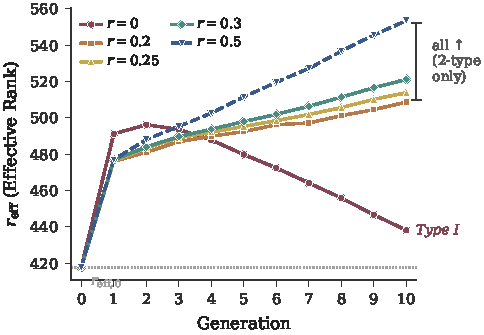
\includegraphics[width=0.92\columnwidth]{figures/rankme_trajectories.pdf}
\caption{Effective rank ($r_{\mathrm{eff}}$) trajectories across mixing ratios. Unlike SLV (Figure~\ref{fig:phase_diagram}), $r_{\mathrm{eff}}$ rises monotonically for all $r \geq 0.2$, providing only a 2-type classification and failing to identify the Type~II transitional regime.}
\label{fig:rankme_trajectories}
\end{figure}

\paragraph{Type~III: Super-critical Mixing ($r \geq 0.3$).}
SLV rises monotonically from Gen~2 onward.
At $r{=}0.3$, SLV reaches 2508.2 at Gen~10 ($+$6.0\% above baseline); at $r{=}0.5$, 2572 ($+$8.7\%).
The critical threshold is robust to EMA smoothing ($\alpha \in \{0.3, 0.5, 0.7\}$ all yield $r_{\text{crit}} \in (0.25, 0.3]$; Appendix Table~\ref{tab:alpha_robustness}), and the maximum SLV departure below baseline (multi-seed mean) shrinks continuously with $r$ ($-7.3$ at $r{=}0.2$, $-3.3$ at $r{=}0.25$, $-1.5$ at $r{=}0.3$), consistent with a continuous crossover.
$r_{\text{crit}}$ thus marks a transition in trajectory shape, not in final outcome: Type~II trajectories recover spectrally but exhibit an initial contraction transient that Type~III trajectories lack.

\paragraph{Output Diversity Divergence.}
D-4 does not increase monotonically with $r$: it remains highest around $r \in \{0.2, 0.25\}$ (mean $.324$--$.342$, with high cross-seed variance s.d.\ $\approx 0.17$) before dropping to .152 at $r{=}0.5$: spectral expansion does not guarantee diversity.
D-4 also shows substantially higher cross-seed variance than SLV (CV $= 3.9\%$ vs.\ $0.12\%$ at $r{=}0.25$); the two metrics capture orthogonal aspects of model behavior.

Table~\ref{tab:phase_summary} consolidates the final-generation metrics across all five mixing ratios.

\paragraph{Practical Implications.}
Neither second-order acceleration ($\Delta^2_t$, Eq.~\ref{eq:second_order}) nor level-based triggers resolve the attenuation problem: $\Delta^2_t$ is negative in late generations regardless of $r$, and level-based triggers fail under Type~III.
The trajectory map provides a direct prescription: setting $r > 0.3$ prevents spectral collapse without per-generation monitoring.

\begin{table}[t]
\centering
\small
\setlength{\tabcolsep}{4pt}
\begin{tabular}{@{}cccccccc@{}}
\toprule
$r$ & Type & SLV & $r_{\text{eff}}$ & PPL & D-4 & $\max\Delta_t$ & Gen. \\
\midrule
0    & I   & 2181.4 & 438.1 & 71.0\phantom{0} & .324 & ---   & 10 \\
0.20 & II  & 2467.2 & 508.1 & 13.54 & .324 & .0016 & 10 \\
0.25 & II  & 2488.1 & 513.8 & 13.41 & .342 & .0005 & 10 \\
0.30 & III & 2508.2 & 521.1 & 13.34 & .295 & 0     & 10 \\
0.50 & III & 2571.6 & 553.5 & 15.11 & .152 & 0     & 10 \\
\bottomrule
\end{tabular}
\caption{Final-generation spectral and downstream metrics across mixing ratios (all runs to Gen~10). PPL = perplexity, D-4 = distinct-4. $\max\Delta_t$ computed for $t \geq 2$, excluding the initial fine-tuning transient. Type classification follows \S\ref{subsec:phase_diagram}. $r{=}0$ reports the mean of three seeds (42, 43, 44); $r{=}0.3$ the mean of three seeds (42, 43, 44); $r{=}0.2$ the mean of three seeds (42, 43, 44); $r{=}0.5$ the mean of two seeds (42, 43; $n{=}2$ precludes reliable uncertainty estimation); $r{=}0.25$ the mean of three seeds (42, 43, 44). D-4 exhibits high cross-seed variance at $r{=}0$ (s.d.\ $= 0.15$) and $r{=}0.3$ (s.d.\ $= 0.155$).}
\label{tab:phase_summary}
\end{table}

\subsection{Cross-Architecture Validation}
\label{subsec:cross_arch}

To test whether the three-phase trajectory generalizes beyond Pythia, we repeat the recursive pipeline on GPT-2-medium~\citep{radford2019language} (355M parameters, different pretraining corpus and tokenizer) under four conditions: pure synthetic ($r{=}0$, 9 generations), intermediate mixing ($r{=}0.25$ and $r{=}0.3$, 3 generations each), and a real-data control ($r{=}1.0$, 3 generations).

Under pure synthetic training, GPT-2-medium reproduces the three-phase pattern (Table~\ref{tab:cross_arch}): SLV peaks at Gen~2 (924, $+$34.1\% from baseline) and declines to 415 by Gen~9 ($-$55.1\% from peak), while perplexity rises from 15.5 to 329 ($+$2028\%).
The $\sigma_1$ trajectory follows the same U-shape (6598$\to$1191 during decompression, rising to ${\sim}$1570 by Gen~9); dominant-direction reconcentration under falling effective rank is architecture-independent.
The collapse magnitude is substantially larger than Pythia's ($-$55.1\% vs.\ $-$11.6\% SLV decline), consistent with GPT-2-medium's more anisotropic initial spectrum ($r_{\text{eff}}{=}23$ vs.\ Pythia's 418).

The real-data control ($r{=}1.0$) shows monotonic expansion with perplexity \emph{decreasing} ($-$27.4\%), which confirms that collapse is specific to recursive synthetic training.

At intermediate ratios ($r{=}0.25$, $r{=}0.3$), both conditions reproduce the decompression phase (Gen~0$\to$1: SLV $+$7.5--8.5\%, $r_{\text{eff}}$ from 23 to 136--142, $\sigma_1$ $-$80--82\%) and stabilize through Gen~3, with EMA-smoothed SLV monotonically non-decreasing.
At $r{=}0.3$ this matches Pythia's Type~III classification.
At $r{=}0.25$, the three-generation window does not resolve the Type~II/III distinction, since Pythia's characteristic EMA dip appears only at Gen~5+; the trajectory is consistent with the Pythia-410M phase boundary but does not independently confirm $r_{\text{crit}}$ for this architecture.

\begin{table}[t]
\centering
\small
\setlength{\tabcolsep}{4pt}
\begin{tabular}{@{}cccccc@{}}
\toprule
$r$ & Type & SLV$_0$ & SLV$_{\text{end}}$ & $\Delta$SLV & Match \\
\midrule
0    & I    & 689  & 415\,(G9)  & $-$39.8\% & \checkmark \\
0.25 & ---  & 689  & 738\,(G3)  & $+$7.0\%  & $\dagger$ \\
0.30 & III  & 689  & 737\,(G3)  & $+$6.9\%  & \checkmark \\
1.0  & Ctrl & 689  & 813\,(G3)  & $+$17.9\% & \checkmark \\
\bottomrule
\end{tabular}
\caption{Cross-architecture validation on GPT-2-medium (355M, seed~42). \textbf{Match}: whether the trajectory type matches the corresponding Pythia-410M classification. $\dagger$\,Three-generation horizon does not resolve the Type~II/III distinction at this ratio.}
\label{tab:cross_arch}
\end{table}
